\documentclass[11pt, letterpaper]{article}

%% ── Packages ──────────────────────────────────────────────────────────────
\usepackage[margin=1in]{geometry}
\usepackage{fontenc}
\usepackage[utf8]{inputenc}
\usepackage{microtype}
\usepackage{parskip}
\usepackage{titlesec}
\usepackage{xcolor}
\usepackage{graphicx}
\usepackage{booktabs}
\usepackage{enumitem}
\usepackage{hyperref}
\usepackage{amsmath}
\usepackage{array}
\usepackage{mdframed}
\usepackage{setspace}
\usepackage{caption}
\usepackage{tikz}
\newcommand{\circled}[1]{\tikz[baseline=(char.base)]{\node[shape=circle,draw,inner sep=1.2pt,font=\small\bfseries] (char) {#1};}}

%% ── Colors ────────────────────────────────────────────────────────────────
\definecolor{lumenblue}{HTML}{1565C0}
\definecolor{shapepurp}{HTML}{6A1B9A}
\definecolor{sortorang}{HTML}{BF360C}
\definecolor{crossgreen}{HTML}{1B5E20}
\definecolor{synthgray}{HTML}{37474F}
\definecolor{scimlindigo}{HTML}{1A237E}
\definecolor{lightgray}{HTML}{F5F5F5}
\definecolor{rulecolor}{HTML}{DDDDDD}

%% ── Section formatting ────────────────────────────────────────────────────
\titleformat{\section}[block]
  {\large\bfseries\color{white}}
  {}
  {0pt}
  {\colorbox{lumenblue}{\parbox{\dimexpr\linewidth-2\fboxsep}{\thesection\quad #1}}}

% Redefine per-project with colors via manual approach (starred sections)
\newcommand{\projectsection}[2]{%   #1=color, #2=title
  \vspace{1.5em}
  {\large\bfseries\color{white}%
   \colorbox{#1}{\parbox{\dimexpr\linewidth-2\fboxsep\relax}{\strut\quad #2\strut}}}\par
  \vspace{0.4em}
}

\titleformat{\subsection}[runin]
  {\normalsize\bfseries\scshape\color{black}}
  {}
  {0pt}
  {}[.\quad]

\titleformat{\subsubsection}[runin]
  {\normalsize\bfseries\color{black}}
  {}
  {0pt}
  {}[.\quad]

%% ── Status badge ──────────────────────────────────────────────────────────
\newcommand{\status}[1]{%
  \textit{\small\color{gray} [#1]}%
}

%% ── Figure environment wrapper ────────────────────────────────────────────
\newenvironment{schematic}[1]{%
  \begin{mdframed}[backgroundcolor=lightgray, linecolor=rulecolor,
                   linewidth=0.8pt, innertopmargin=8pt, innerbottommargin=6pt]
  \centering
}{%
  \end{mdframed}
}

%% ── Hyperref setup ────────────────────────────────────────────────────────
\hypersetup{
  colorlinks=true,
  linkcolor=scimlindigo,
  urlcolor=scimlindigo,
  pdftitle={Research Project Summaries},
  pdfauthor={Explanatory Modeling Program}
}

%% ── Spacing ───────────────────────────────────────────────────────────────
\setlength{\parskip}{5pt}
\setlength{\parindent}{0pt}

%% ═══════════════════════════════════════════════════════════════════════════
\begin{document}

\begin{center}
  {\LARGE\bfseries Research Project Summaries}\\[0.4em]
  {\large Explanatory Modeling Program --- hiPSC Lumenoid Morphogenesis}\\[0.3em]
  {\small\color{gray} \today}
\end{center}
\vspace{0.5em}
\hrule
\vspace{1em}

%% ── Overarching Goal ──────────────────────────────────────────────────────
\textbf{Overarching Goal.} Relate lumenoid growth, cell movement, and multicellular organization to the active and passive forces---adhesion, actomyosin contractility, cell growth, and proliferation---that generate them. Tissue shape, cell dynamics, and sorting are expressed through a unified \textit{cell state representation} linking molecular perturbations to tissue-scale observables.

\textbf{Explanatory Modeling Framework.} The program runs in two phases. In the \textit{hypothesis-driven phase} (now), fast cycles of experiment $\to$ segmentation/tracking $\to$ hypothesis $\to$ forward model identify dominant physical parameters. In the \textit{scientific ML phase}: \textbf{Phase~2a} (parameter inference, near-term) takes known model forms and infers constitutive parameters from data; \textbf{Phase~2b} (equation discovery, longer-term, contingent on the label-free pipeline under development) discovers which terms and fields govern dynamics without assuming the model form. Running either stage across the perturbation series triangulates the cell ``energy'' or state landscape.

\begin{schematic}{}
  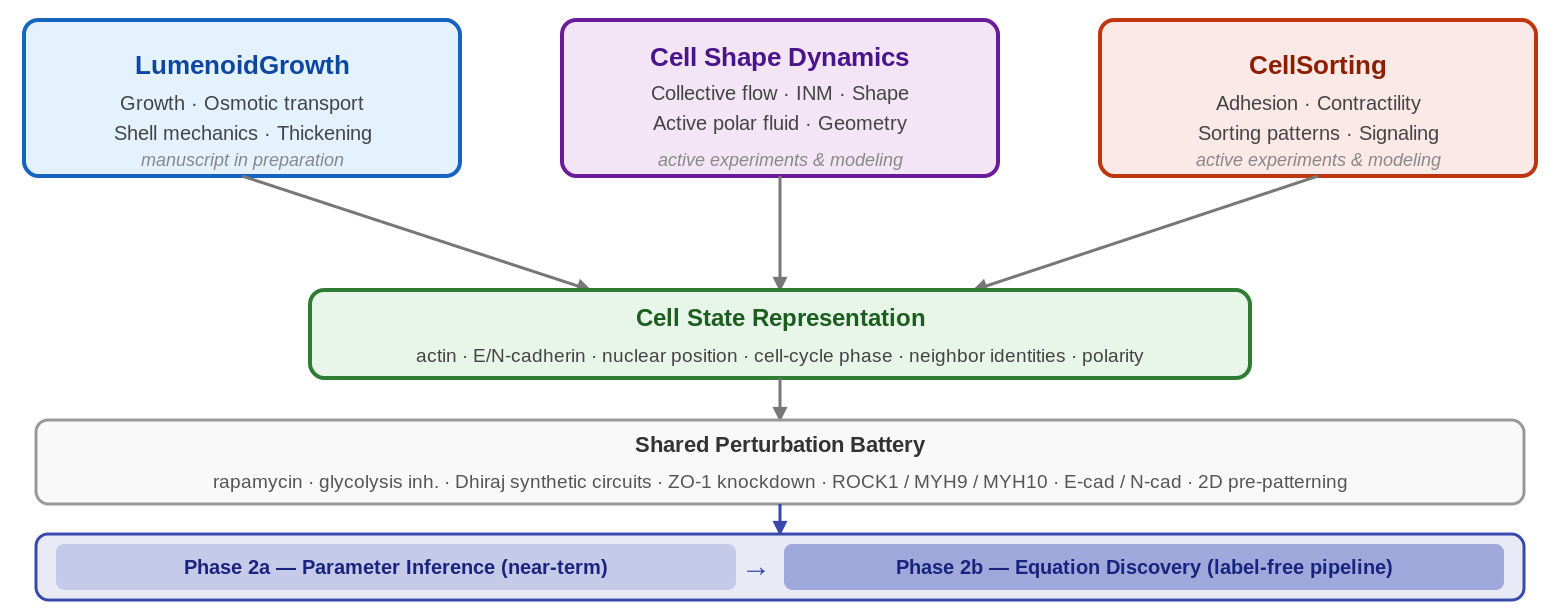
\includegraphics[width=\linewidth]{figures/fig1.png}
  \captionof*{figure}{\textbf{Figure~1.} Program architecture. Three projects share a common cell state representation, perturbation battery, and scientific ML pipeline (Phase~2a $\to$ Phase~2b).}
\end{schematic}

\vspace{1em}\hrule

%% ═══════════════════════════════════════════════════════════════════════════
\projectsection{lumenblue}{LumenoidGrowth}
\status{manuscript in preparation}

\subsection{Measure}
Time-lapse imaging tracks inner radius, outer radius, and epithelial thickness over days. The central observation---the epithelium \textit{thickens} while the lumen grows, opposite to pressure-driven thinning in most organoids---is quantified across control, rapamycin, and TJP1/ZO-1 CRISPRi knockdown. The next layer adds mosaic TJP1 lumenoids, DOX washout experiments (competing timescales), and actomyosin perturbations. \textbf{Actin and E-cadherin/N-cadherin intensity fields} connect cytoskeletal organization and adhesion to shell mechanics. Growth rate is controlled via three independent routes: \textbf{rapamycin} (mTOR), \textbf{glycolysis inhibitors} (2-DG; distinct metabolic node), and \textbf{Dhiraj's synthetic growth control circuits} (direct cell-cycle). All three should produce matched thickness reductions when calibrated by rate; deviations reveal pathway-specific effects.

\subsection{Model}
The \textbf{manuscript} rests on a minimal continuum model coupling (1) cell volume growth, (2) osmotic transport, and (3) elastic shell mechanics. Key insight: when growth outpaces osmotic and elastic relaxation, area compression converts to thickness increase via cell incompressibility; the lumenoid operates in a \textit{strong osmotic flow} regime. Post-publication, the continuum model extends to \textbf{Voronoi/vertex models} resolving individual cells---the natural target for Phase~2a SciML.

\begin{schematic}{}
  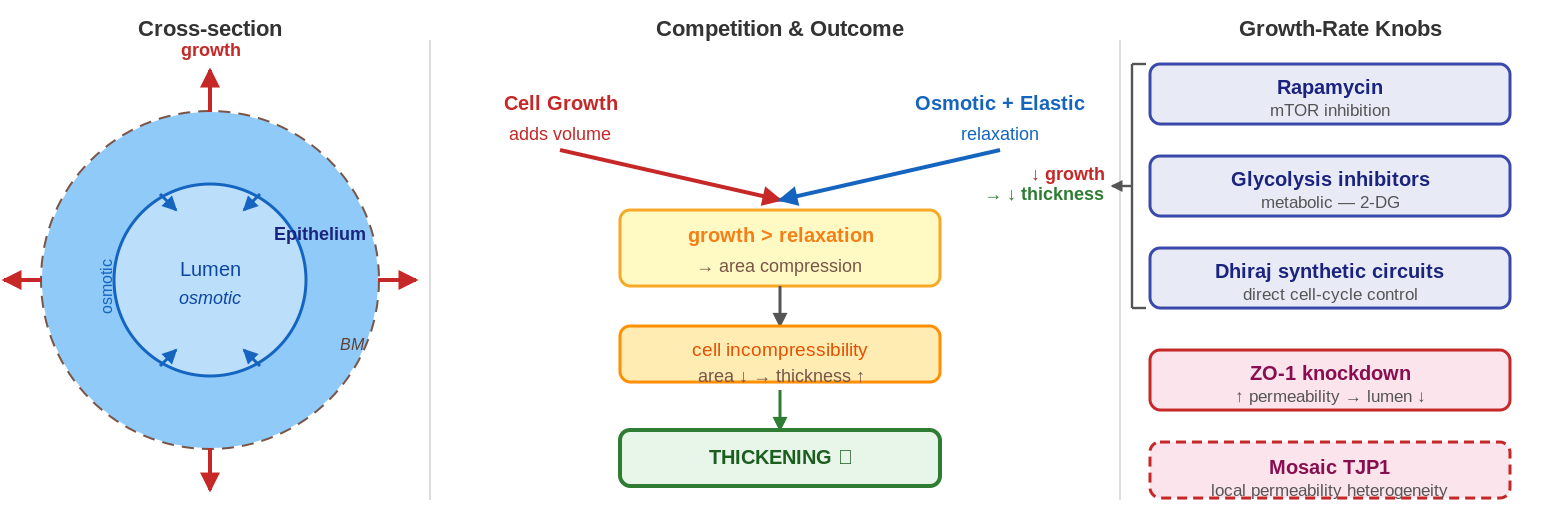
\includegraphics[width=\linewidth]{figures/fig2.png}
  \captionof*{figure}{\textbf{Figure~2.} LumenoidGrowth mechanism. Left: lumenoid cross-section with growth (red outward arrows) and osmotic transport (blue inward arrows). Center: competition between growth and relaxation produces area compression, which cell incompressibility converts to thickening. Right: three independent growth-rate knobs and osmotic perturbations.}
\end{schematic}

\subsection{Predict}
(1)~Faster growth $\to$ thicker shell (validated). (2)~Increasing permeability shrinks lumen strongly (strong-flow regime, validated). (3)~All three growth-rate methods should produce matched thickness reductions. (4)~DOX washout reveals the timescale hierarchy between osmotic and elastic relaxation. (5)~Actomyosin perturbations change effective stiffness independently of growth rate.

\subsection{Build / Validate}
Continuum model maps the growth rate $\times$ permeability parameter space. Validated: control, rapamycin, ZO-1. Open: single-cell volume measurements, mosaic and actomyosin datasets, post-publication vertex model.

\vspace{1em}\hrule

%% ═══════════════════════════════════════════════════════════════════════════
\projectsection{shapepurp}{Cell Shape Dynamics}
\status{active experiments and model development}

\subsection{Measure}
\textbf{Collective motion:} 2D colonies show coherent CCW rotation (label-free brightfield). On the 3D surface (lattice light-sheet, LLS), nuclear velocity fields form vortices and spirals with point-source cores. \textbf{Cell/nuclear shape:} flat/cuboidal in 2D $\to$ columnar/pseudostratified in 3D. The \textit{apical-basal nuclear motion} track resolves z-displacement as a function of cell-cycle phase from existing LLS data. \textbf{Molecular fields:} actin intensity (polarity proxy), E-cadherin and N-cadherin (adhesion landscape, alternative force descriptors). \textbf{Perturbations:} rapamycin/glycolysis inhibitors/Dhiraj circuits; ZO-1 and mosaic ZO-1; ROCK1/MYH9/MYH10; E-cad/N-cad induction. \textbf{48-hour LLS runs} ($>$1 division) will resolve nuclear volume, cell count, streamlines vs.\ size $R$, and INM-streamline correlation. \textbf{2D pre-patterning:} prior experiments confirm stripes seed hollow cylinders with two spherical caps and concentric rings seed toroidal lumenoids.

\begin{schematic}{}
  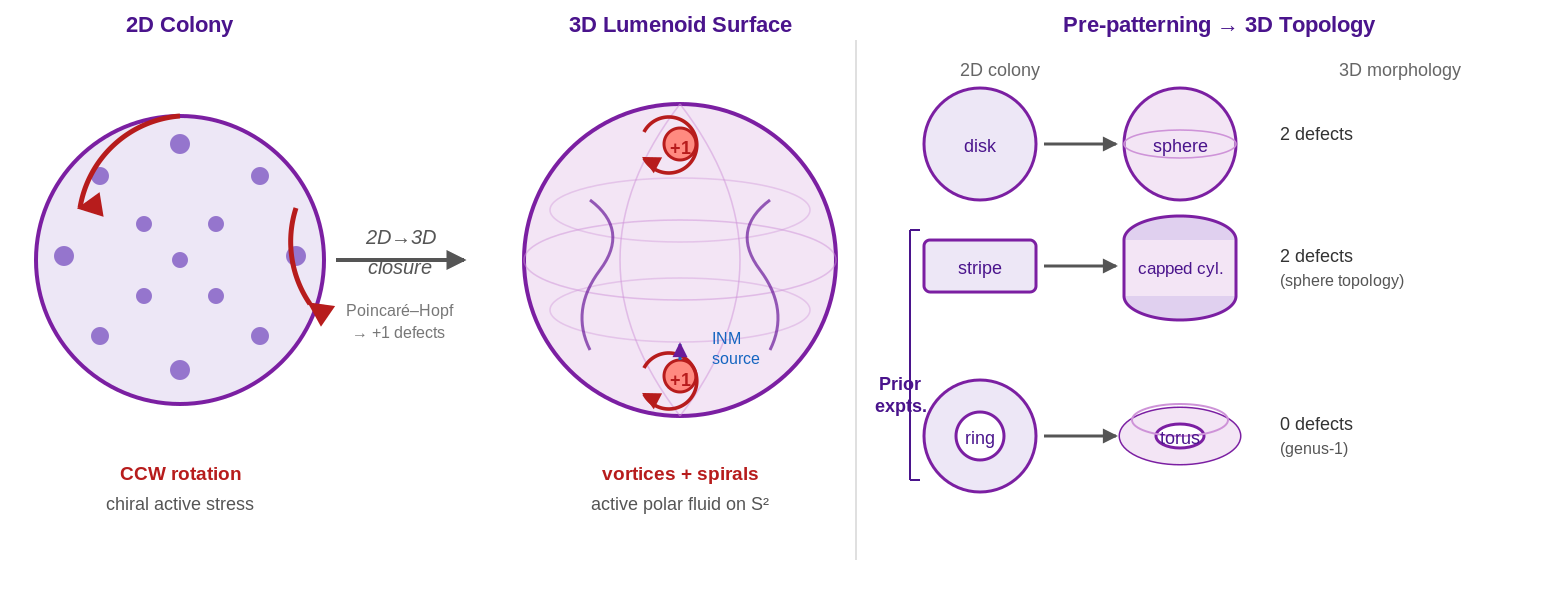
\includegraphics[width=\linewidth]{figures/fig3.png}
  \captionof*{figure}{\textbf{Figure~3.} 2D CCW rotation $\to$ 3D vortices/spirals (Poincar\'e--Hopf forces $+1$ defects; INM provides the surface-divergence source). Right: pre-patterning geometry controls 3D topology---disk seeds sphere (2 defects), stripe seeds capped cylinder (2 defects, sphere topology), ring seeds torus (genus-1).}
\end{schematic}

\subsection{Model}
Three complementary frameworks:

\textit{Active polar fluid (continuum, current default).} Chiral active polar/nematic gel on $S^2$; active driving force $\mathbf{f} = \gamma v_0 \mathbf{p}$ (monopolar traction). Pure in-plane incompressible flow yields only closed vortex loops; spirals require out-of-plane INM as a surface divergence source. Solved pseudospectrally (IMEX, toroidal $+$ spheroidal on $S^2$).

\textit{Voronoi/vertex model (cell-resolved).} Extended with polarity dynamics and active traction; suited for mosaic perturbations and cell-cycle-gated events.

\textbf{Shape Dynamics} (\textit{Langevin subproject}).\ Each cell/nucleus is decomposed into spherical harmonic or PCA shape coefficients $\mathbf{q} = (q_1,\ldots,q_n)$, modeled as:
\begin{equation*}
  \frac{dq_i}{dt} = -\frac{\partial E(\mathbf{q},\,\text{neighbor states})}{\partial q_i} + \eta_i(t)
\end{equation*}
Fitting to tracked shape trajectories infers $E(\mathbf{q})$ and noise statistics directly from data.

\textit{Phase~2a SciML:} given $\mathbf{v}(\mathbf{x},t)$, actin $I_a(\mathbf{x},t)$, cadherin $I_c(\mathbf{x},t)$, learn $I_a \to \mathbf{p}$ and infer $\zeta, \kappa, K, \gamma v_0$ via sparse regression or PINNs. \textit{Phase~2b:} discover governing equations without assumed model form (contingent on label-free data scale-up).

\begin{schematic}{}
  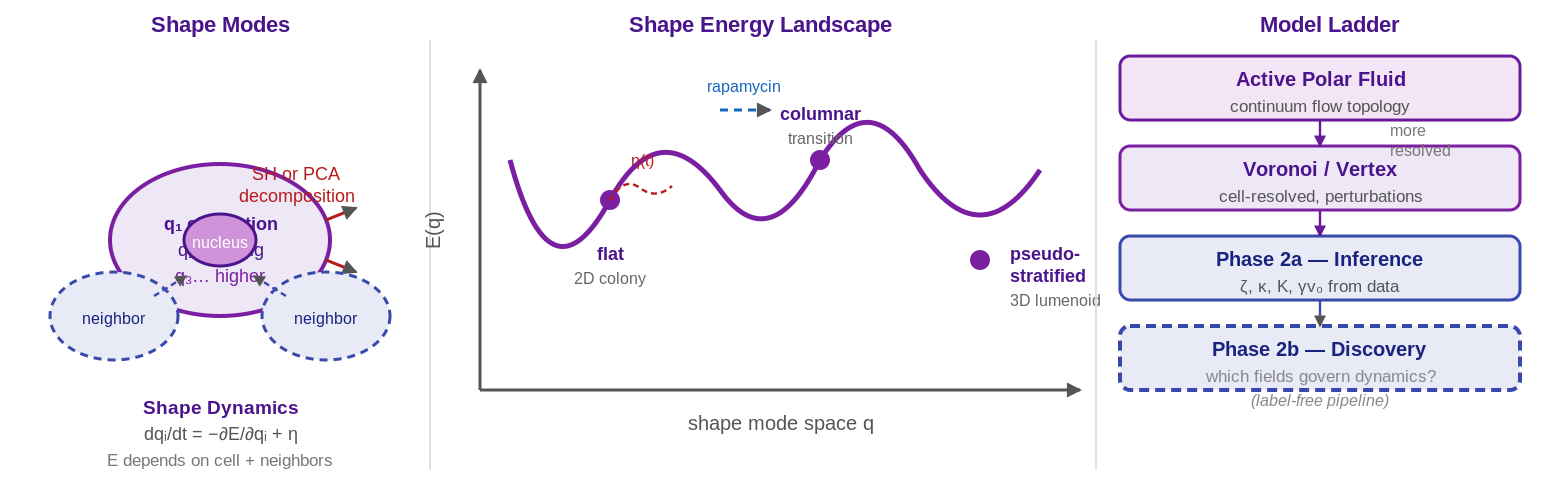
\includegraphics[width=\linewidth]{figures/fig4.png}
  \captionof*{figure}{\textbf{Figure~4.} Shape Dynamics subproject and model resolution ladder. Left: shape mode decomposition and neighbor coupling. Center: energy landscape with flat/columnar/pseudostratified wells. Right: four model levels from continuum active polar fluid to Phase~2b equation discovery.}
\end{schematic}

\subsection{Predict}
(1)~$\omega(r)$ rescales with colony size/screening length; chirality reversal reverses both 2D rotation sense and 3D spiral handedness. (2)~Surface divergence $\nabla_S \cdot \mathbf{v}$ localized at spiral cores; blocking INM converts spirals to vortices. (3)~Streamline topology changes with $R$ near-parameter-freely. (4)~All three growth-rate perturbations reduce flow magnitude and spiral intensity. (5)~Actin intensity correlates with polarity field throughout tissue (monopolar) not just near defects (dipolar). (6)~Stripe-seeded capped cylinders (sphere topology, $\chi=2$, 2 defects) and ring-seeded toroids ($\chi=0$, 0 defects) show qualitatively different defect arrangements from geometry alone, even though the sphere and capped cylinder share the same defect count. (7)~Low-order shape modes have longer relaxation times; neighbor shape correlations are detectable. (8)~Phase~2a inferred parameters co-vary low-dimensionally if a single cell state variable underlies them.

\subsection{Validate}
Solver validated (9/9 tests); point-source Green's function reproduced to $<10^{-3}$. Sequence: (i)~$\omega(r)$ profile vs.\ active-nematic prediction; (ii)~surface divergence at spiral cores; (iii)~size-$R$ scaling from 48-hr runs; (iv)~INM-streamline correlation; (v)~actin/cadherin field correlations with velocity; (vi)~geometry experiments; (vii)~Phase~2a parameters on theoretical phase diagram; (viii)~Langevin $E(\mathbf{q})$ predictions on held-out data.

\vspace{1em}\hrule

%% ═══════════════════════════════════════════════════════════════════════════
\projectsection{sortorang}{CellSorting}
\status{active experiments and model development}

\subsection{Measure}
Two hiPSC populations in a lumenoid; one carries DOX-inducible N-cadherin. Measurement battery: membrane-localized N-cadherin and \textbf{E-cadherin intensity} (endogenous baseline), heterotypic contact fraction, domain interface length, neighbor-exchange rate, cell MSD, pattern autocorrelation, and \textbf{actin intensity} (contractility readout). Immediate priority: \textbf{DOX washout kinetics}---fit $dN/dt = k_{\rm on} f(C_{\rm DOX}) - k_{\rm off} N$. Second layer: \textbf{pattern reversibility} at partial, mature, and full sorting. Third layer: \textbf{actomyosin perturbations} (ROCK1, MYH9, MYH10 via iCRISPRi; blebbistatin, Y-27632).

\subsection{Model}
Dynamical self-organization: cell state $\to$ adhesion/contractility/motility $\to$ rearrangement $\to$ new neighbors $\to$ signaling/state. Immediate model: \textbf{Voronoi/vertex simulation} with time-dependent adhesion, independent edge tension $\Lambda_{ij}(t)$, and proliferation. Phase~2a SciML infers $E(\text{cell state})$ from N-cadherin, E-cadherin, and actin fields. Longer-term: \textbf{neighbor-dependent signaling} closes the mechanics-signaling feedback loop.

\begin{schematic}{}
  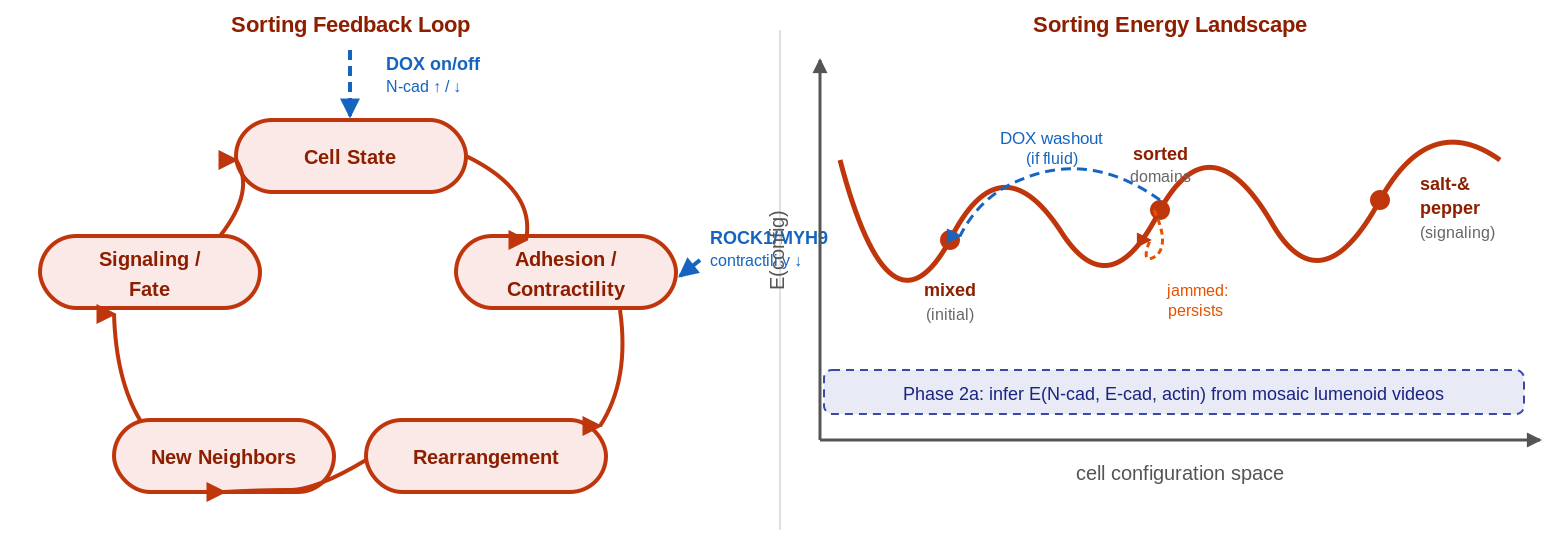
\includegraphics[width=\linewidth]{figures/fig5.png}
  \captionof*{figure}{\textbf{Figure~5.} CellSorting feedback loop (left) and energy landscape (right). DOX washout either remixes (fluid tissue) or remains trapped (jammed); Phase~2a SciML infers $E$ from molecular intensity fields.}
\end{schematic}

\subsection{Predict / Build / Validate}
(1)~Fluid lumenoids remix after washout; jammed lumenoids retain domains---persistence correlates with neighbor-exchange rate, not instantaneous sorting index. (2)~MYH9 and MYH10 knockdowns produce distinct interface phenotypes. (3)~Phase~2a inferred landscape: N-cadherin and actomyosin perturbations are orthogonal axes if adhesion and contractility are separable. Current capability: DOX-inducible N-cadherin sorting demonstrated; agent-based models fast enough for parameter sweeps. Open: DOX response model fit, reversibility at partial vs.\ mature sorting, actomyosin perturbation feasibility, Phase~2a validation.

\vspace{1em}\hrule

%% ═══════════════════════════════════════════════════════════════════════════
\projectsection{crossgreen}{Cross-Cutting Themes}

\subsection{Cell State Representation}
All three projects measure overlapping quantities on the same cells: nuclear trajectories, actin intensity, E/N-cadherin levels, cortical tension proxies, cell-cycle phase, and neighbor identities. A unified per-cell state vector encodes these as functions of position and time. A perturbation maps onto a trajectory in this space; tissue-scale outcomes are readouts of that trajectory.

\subsection{Scientific ML Pipeline}

\textbf{Phase~2a---Parameter inference (near-term).} Given $\mathbf{v}(\mathbf{x},t)$, actin $I_a(\mathbf{x},t)$, and cadherin $I_c(\mathbf{x},t)$: learn $I_a \to \mathbf{p}$ and infer $\zeta, \kappa, K, \gamma v_0$ via sparse regression or PINNs. For the vertex model: learn $E(\text{cell state})$. Each perturbation condition produces a point in parameter space; the collection maps the cell energy/state landscape.

\textbf{Phase~2b---Equation discovery (longer-term).} Without assumed model form, sparse regression or PINNs identify which terms are necessary. Answers whether actin, cadherin, mitosis, or combinations are minimal sufficient force descriptors. Contingent on the label-free pipeline reaching sufficient data volume.

\begin{schematic}{}
  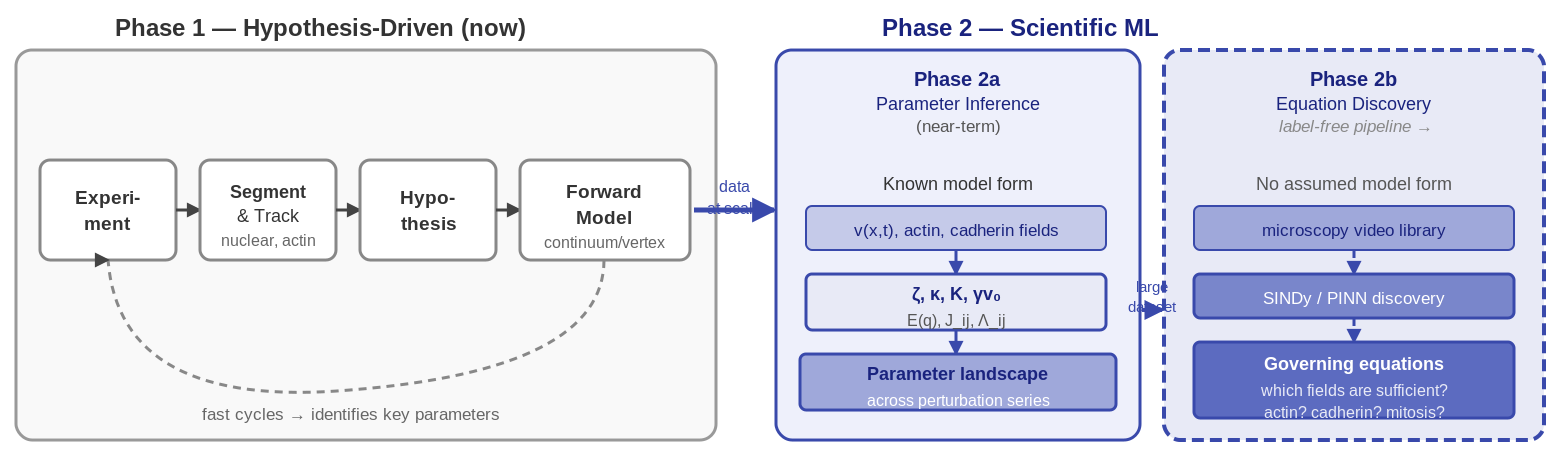
\includegraphics[width=\linewidth]{figures/fig6.png}
  \captionof*{figure}{\textbf{Figure~6.} Scientific ML pipeline. Phase~1: fast hypothesis-driven cycles. Phase~2a: parameter inference from known model forms. Phase~2b: equation discovery at scale (label-free pipeline).}
\end{schematic}

\subsection{Shared Perturbation Logic}
Growth rate via three independent routes: rapamycin (mTOR), glycolysis inhibitors (2-DG), Dhiraj's synthetic circuits (cell-cycle direct). Combined with ZO-1 knockdown (mosaic), actomyosin perturbations (ROCK1, MYH9, MYH10, pharmacological), and E-cad/N-cad induction/washout. Each perturbation is a sampling point in the cell state landscape; new perturbations are new sampling points chosen to maximally discriminate competing model structures.

\subsection{Geometry as a Control Variable}
2D pre-patterning (stripes, concentric disks, squares) changes boundary conditions and global symmetry rather than molecular composition. Prior experiments confirm: stripes seed hollow cylinders with two spherical caps; rings seed toroids. Different geometries impose different defect structures (active polar fluid) and different effective boundary potentials on shape modes (Langevin Shape Dynamics).

\vspace{1em}\hrule

%% ═══════════════════════════════════════════════════════════════════════════
\projectsection{synthgray}{Synthetic Modules}

A major arm of the program designs and deploys synthetic genetic circuits providing precise, tunable, and reversible control over cellular processes. Four functional classes are being developed.

\subsection{Module Classes}

\textbf{\circled{1} Fate control.} Drives cells toward specific identities, polarization states, or differentiation programs. Sets mosaic cell-type composition; biases apical vs.\ basal polarity; gates 2D$\to$3D transition timing.

\textbf{\circled{2} Cell-cell communication.} Implements synthetic intercellular signaling---lateral inhibition (synthetic Delta-Notch), juxtacrine feedback, diffusible sender/receiver pairs. Closes the signaling-mechanics feedback loop modeled in CellSorting. The expressing fraction (sender vs.\ receiver) is a direct tunable parameter.

\textbf{\circled{3} Adhesion and contractility.} Inducible, reversible, dose-controlled access to E-cadherin, N-cadherin (deployed), ROCK1, MYH9, MYH10. Orthogonal inducible promoters (e.g., DOX and abscisic acid) in the same cell enable true independent titration of the adhesion and contractility axes---impossible pharmacologically.

\textbf{\circled{4} Mechano-biological circuits.} Output regulated by mechanical signals---membrane tension, cytoskeletal strain, hydrostatic pressure, curvature. Turn the tissue into a self-reporting system; introduce mechano-biological feedback that can stabilize or destabilize morphogenetic trajectories.

\begin{schematic}{}
  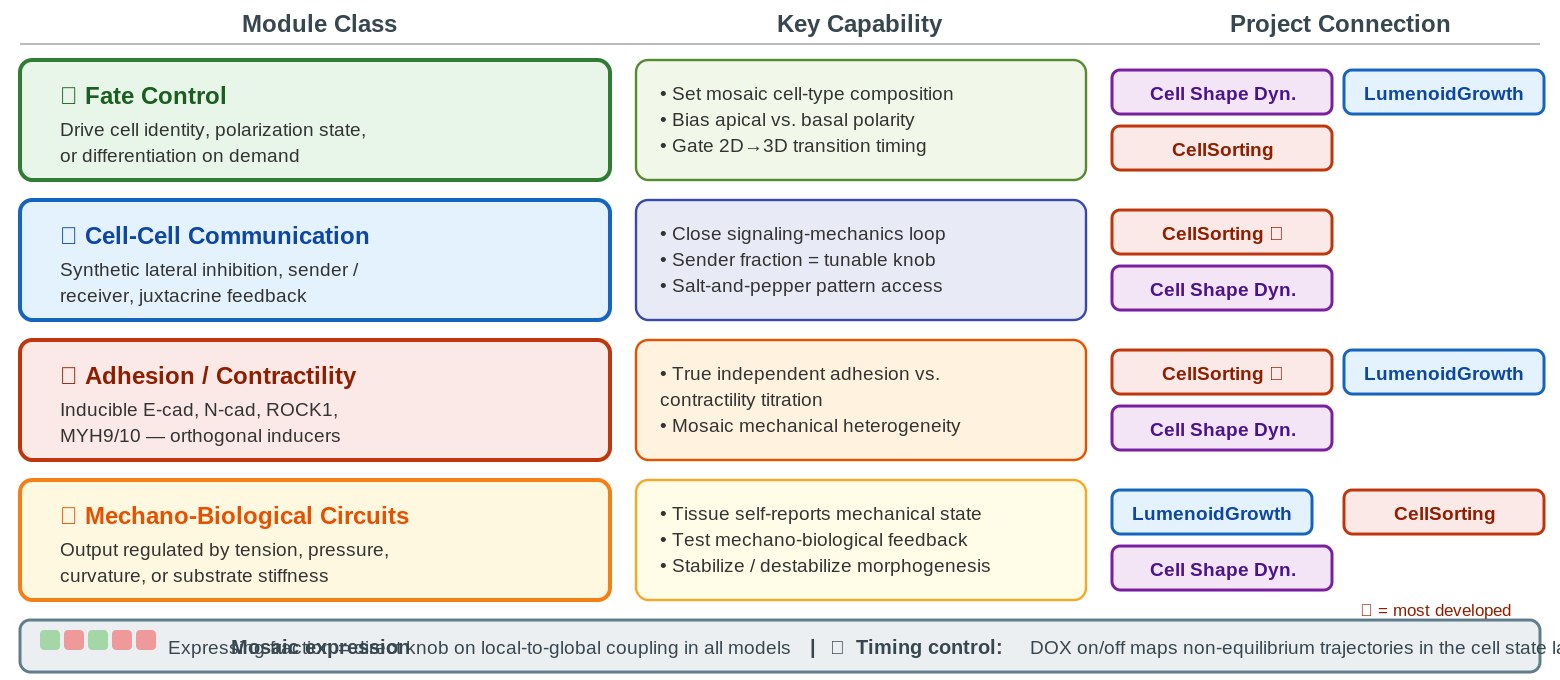
\includegraphics[width=\linewidth]{figures/fig7.png}
  \captionof*{figure}{\textbf{Figure~7.} Synthetic module classes and project connections. Four circuit types contribute to the three projects via perturbation amplitude, mosaic spatial control, and timing. Bottom strip: mosaic expression (expressing fraction as local-to-global coupling knob) and timing control (DOX on/off generates non-equilibrium cell state trajectories) are the two unique cross-cutting capabilities.}
\end{schematic}

\subsection{Connection to Projects}

\textbf{LumenoidGrowth.} Dhiraj's growth circuits are the third independent growth-rate knob. Key additions: (i)~\textit{mosaic growth circuit}---defined expressing fraction tests whether local growth suppression propagates into global shell mechanics; (ii)~\textit{mechano-sensing growth feedback}---circuit reducing growth rate under compressive stress tests whether the tissue regulates its own thickening; (iii)~\textit{synthetic permeability circuit}---inducible claudin/channel expression, cleaner than CRISPRi ZO-1.

\textbf{Cell Shape Dynamics.} A synthetic polarity circuit biasing a defined fraction of cells directly tests how the polarity field $\mathbf{p}$ is established and how a locally injected polarity bias propagates through an active polar fluid. Mechano-sensing circuits responsive to shear or curvature reveal mechano-biological feedback on vortices and spirals. Timing: applying a polarity perturbation before vs.\ after the 2D$\to$3D transition tests whether the transition is gated by the polarity state. Mosaic actomyosin circuits test how local mechanical defects reorganize global topological defect patterns.

\textbf{CellSorting.} Beyond the current DOX-inducible N-cadherin: (i)~synthetic lateral inhibition closes the signaling-mechanics loop, enabling the salt-and-pepper pattern class; (ii)~orthogonal inducible control of adhesion and contractility in the same cell enables true independent navigation of the sorting phase diagram; (iii)~a mechano-sensing contractility circuit---upregulating actomyosin in response to heterotypic contact force---tests whether domain interfaces are actively stabilized by feedback.

\subsection{Mosaic Expression and Timing as Scientific Tools}

\textbf{Mosaic expression} is the most distinctive capability. A mosaic lumenoid tests local-to-global coupling directly: whether the continuum assumption holds (LumenoidGrowth), how locally perturbed cells reorganize global defect topology (Cell Shape Dynamics), and how the expressing fraction shifts the sorting phase diagram (CellSorting). The expressing fraction is a continuous knob that sweeps through parameter space in a single experiment.

\textbf{Timing control} (DOX on/off) accesses not just amplitude but \textit{timing}. In the SciML framework, timed perturbations generate non-equilibrium trajectories in the cell state landscape whose geometry encodes the direction and curvature of $E(\text{cell state})$ near morphogenetic checkpoints---richer constraints than steady-state observations alone.

\end{document}
